\section{Visualizer.cpp File Reference}
\label{Visualizer_8cpp}\index{Visualizer.cpp@{Visualizer.cpp}}
{\tt \#include \char`\"{}Window.h\char`\"{}}\par
{\tt \#include \char`\"{}Implicits.h\char`\"{}}\par
{\tt \#include \char`\"{}Operators.h\char`\"{}}\par
{\tt \#include \char`\"{}Shading.h\char`\"{}}\par
{\tt \#include \char`\"{}Volumes.h\char`\"{}}\par
{\tt \#include \char`\"{}Visualizer.h\char`\"{}}\par
{\tt \#include \char`\"{}Glut\-Headers.h\char`\"{}}\par
{\tt \#include \char`\"{}Random.h\char`\"{}}\par
{\tt \#include \char`\"{}Matrix.h\char`\"{}}\par


Include dependency graph for Visualizer.cpp:\begin{figure}[H]
\begin{center}
\leavevmode
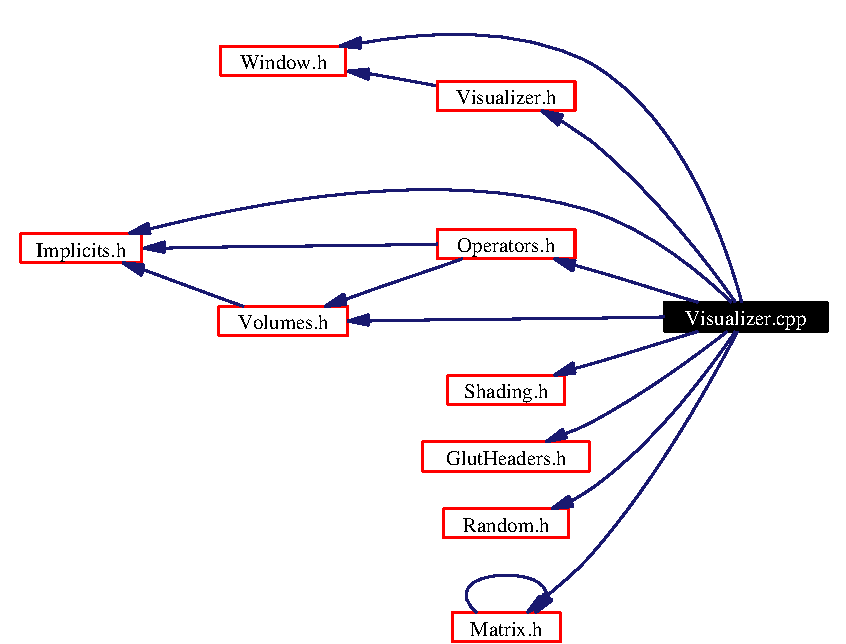
\includegraphics[width=220pt]{Visualizer_8cpp__incl}
\end{center}
\end{figure}
\subsection*{Variables}
\begin{CompactItemize}
\item 
Visualizer {\bf sk\-App}
\end{CompactItemize}


\subsection{Variable Documentation}
\index{Visualizer.cpp@{Visualizer.cpp}!skApp@{skApp}}
\index{skApp@{skApp}!Visualizer.cpp@{Visualizer.cpp}}
\subsubsection{\setlength{\rightskip}{0pt plus 5cm}Visualizer sk\-App}\label{Visualizer_8cpp_a0}




Definition at line 13 of file Visualizer.cpp.